\section{Lettres et pièces de guerre (1916–1918)}\label{annexe-lettres}

Les archives familiales conservent, avec le carnet, quelques pièces autographes de la guerre d'Hippolyte Combes : deux minutes ou copies de lettres de service (1916), une lettre à sa sœur (juin 1916), un poème anglais recopié, et la correspondance adressée à sa femme au lendemain de l'armistice (novembre–décembre 1918). Elles sont transcrites intégralement, d'après les numérisations, selon les principes du carnet (orthographe, ponctuation et abréviations conservées ; changements de page signalés entre crochets) ; une page de chacune est reproduite.


\subsection{Copie autographe d'une lettre d'Hippolyte Combes à un capitaine, ancien camarade de la Faculté de Toulouse, « Au front », 25 février 1916}
\phantomsection\label{annexe:doc1}
\begin{figure}[tbp]\centering
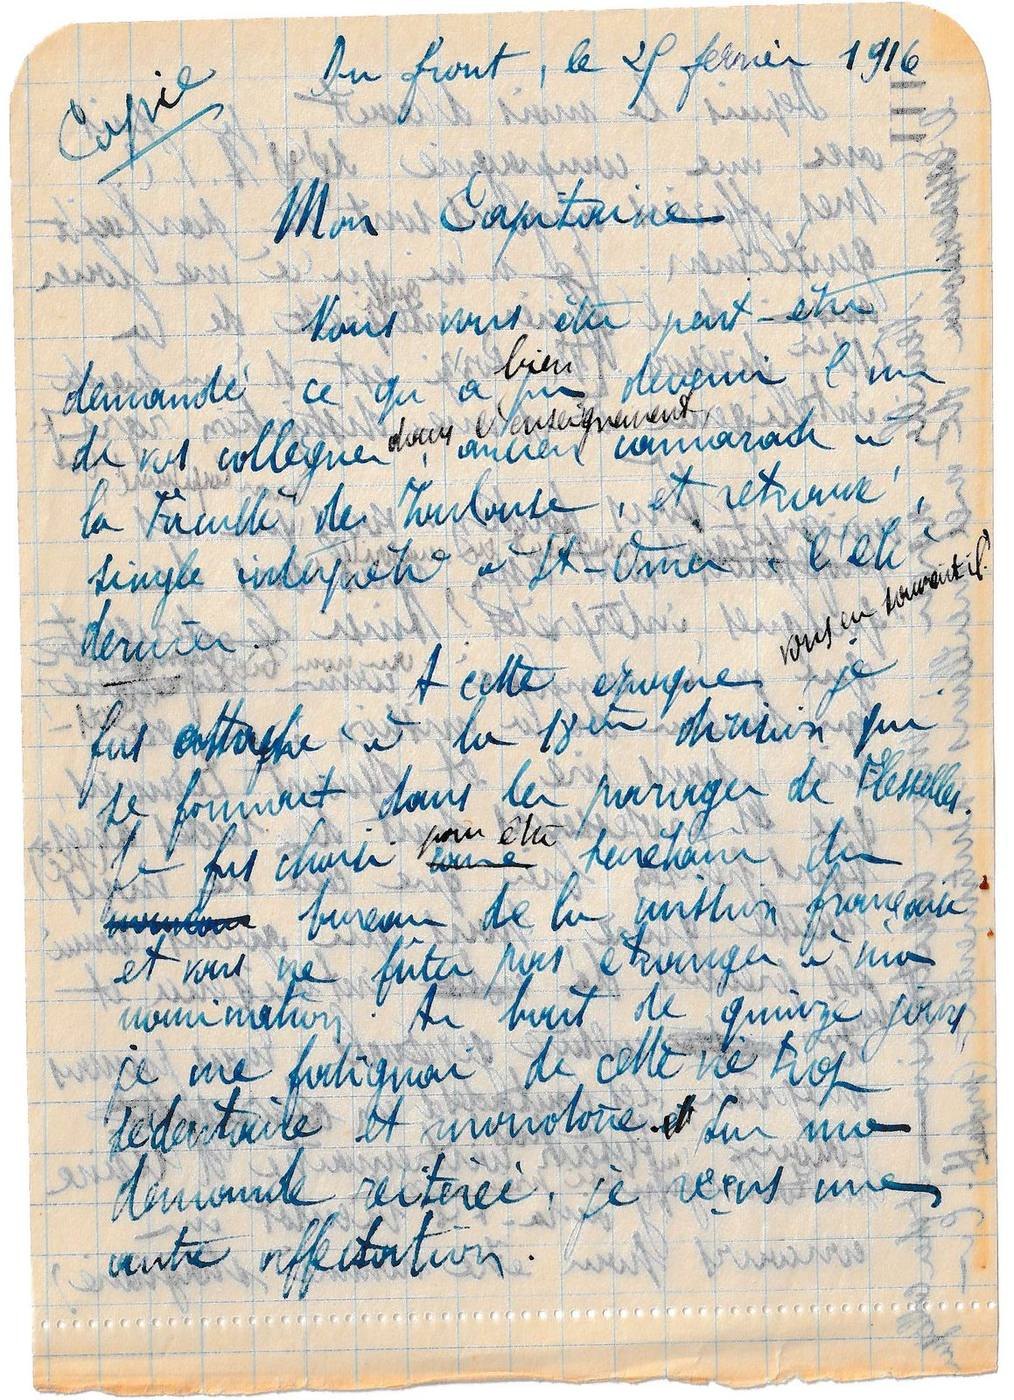
\includegraphics[width=0.78\textwidth,height=0.62\textheight,keepaspectratio]{illustrations/lettres/doc1_fevrier_1916_p1.jpg}
\caption{Copie autographe d'une lettre d'Hippolyte Combes à un capitaine, ancien camarade de la Faculté de Toulouse, « Au front », 25 février 1916, première page (archives familiales).}
\end{figure}

Un feuillet de papier quadrillé (carreaux d'environ 6~mm), d'environ 121~mm de large sur 169~mm de haut, écrit en hauteur au recto et au verso ; les deux coins supérieurs sont arrondis et le bord inférieur, perforé et déchiré, montre que le feuillet a été détaché d'un carnet. Le fichier numérique compte trois vues : les vues 1 et 2 sont deux prises du recto, la vue 3 donne le verso. Le texte est écrit à l'encre bleue (plume à tremper, traits tour à tour chargés et pâlis) ; une seconde campagne, à l'encre noire, ajoute des mots dans l'interligne (« bien », « dans l'enseignement », « pour être », « mon Capitaine ! », « pourtant en majorité », « — un nom bien français — », « un vrai primaire »), rature (« aussi ») et repasse quelques lettres (date, « Copie », « d'A. S. C. », « M. »). La formule finale et les initiales occupent, verticalement, la marge gauche du verso. Un chiffre romain « III » à l'encre noire (tracé à empattements, peut-être tamponné) figure en haut à gauche du verso : c'est une cote de classement postérieure. Bon état ; papier jauni, bords brunis ; la transparence de l'encre gêne par endroits la lecture. Le mot « Copie », en tête, et les corrections indiquent qu'il s'agit du double gardé par Combes (ou d'un brouillon recopié ensuite) d'une lettre réellement envoyée ; la lettre expédiée n'est pas connue. Le destinataire n'est pas nommé : un capitaine que Combes a connu étudiant à la Faculté (des lettres) de Toulouse (« ancien camarade »), lui aussi enseignant (« vos collègues dans l'enseignement »), retrouvé à Saint-Omer à l'été 1915 et qui, d'après la lettre, eut part à la nomination de Combes au bureau de la mission française de la 18\textsuperscript{e}~division ; il appartenait donc vraisemblablement à la Mission militaire française attachée à l'armée britannique, dont Saint-Omer, siège du grand quartier général britannique, était le centre. Son nom ne figure pas sur le document ; aucune identification n'est proposée. La date est lue 25 et non 21 (voir la note). La transcription suit les paragraphes de l'original ; les ajouts à l'encre noire sont signalés en note.

\begin{LJlettre}
\LJsl{Copie}\footnote{« Copie » est souligné d'un seul trait oblique à l'encre bleue (l'édition antérieure : double soulignement) ; le i et son point sont repassés à l'encre noire.} \hfill Au front, le 25\footnote{Le second chiffre a une longue haste descendant sous la ligne, coiffée d'une boucle fermée à droite : c'est le 5 « en ſ », à boucle de tête, de Combes (comparer le 5 du \textit{Livre-Journal}, clichés 002 et 053), alors que le 1 de cette main (1916, 18\textsuperscript{e}) est une haste courte sans boucle. L'édition antérieure lit « 21 ». Le 2, « evrier » et 1916 sont repassés à l'encre noire, sans correction.} fevrier 1916

Mon Capitaine

Vous vous ête\footnote{Circonflexe visible ; aucun s final.} peut-être demandé ce qu a\footnote{Sans apostrophe.} \LJadd{bien}\footnote{Ajout à l'encre noire, au-dessus de « pu ».} pu devenir l'un de vos \LJinc{collegues}\footnote{La finale se réduit à un délié ; le s est douteux et aucun accent n'est visible.} \LJadd{dans l'enseignement}\footnote{Ajout à l'encre noire : « dans » sur la ligne, « l'enseignement » dans l'interligne au-dessus de « ancien ». L'édition antérieure lit « de l'enseignement ».}, ancien camarade à la Faculté de Toulouse, et retrouvé, simple interprète à St-Omer\footnote{Saint-Omer (Pas-de-Calais), siège du grand quartier général britannique (GHQ) d'octobre 1914 à mars 1916 ; les interprètes français affectés à l'armée britannique y passaient avant d'être répartis dans les unités.}, l'été dernier. \LJadd{vous en souvient il.}\footnote{Ajout à l'encre noire, écrit en diagonale montante dans le blanc qui suit « dernier. » ; v minuscule, pas de trait d'union, point final (l'édition antérieure : « Vous en souvient-il ? »).}

A cette époque, je fus attaché à la 18\LJsup{e} division\footnote{Après 18, un e suivi d'un jambage à crochet (même graphie au verso, « (18\textsuperscript{e} ») : abréviation de « dix-huitième » ; cf. « 18\textsuperscript{ie} » du \textit{Livre-Journal}, cliché 095. La 18th (Eastern) Division, division de la «~nouvelle armée~» de Kitchener, débarquée en France en juillet 1915 ; elle se concentra autour de Flesselles (Somme), au nord d'Amiens. C'est l'unité à laquelle Combes est attaché dans le \textit{Livre-Journal}.} qui se formait dans les parages de Flesselles. Je fus choisi \LJdel{comme} \LJadd{pour être}\footnote{« comme », à l'encre bleue, est biffé à l'encre noire ; « pour être » est écrit au-dessus à l'encre noire.} secretaire du \LJdel{membre}\footnote{Mot biffé d'une rature épaisse terminée en crosse ; lecture probable (six minimes, boucle, r, e). L'édition antérieure lit « secrétaire au [membre] bureau » ; le texte porte « du ».} bureau de la mission française\footnote{Le bureau de la Mission militaire française auprès de la division britannique, dirigé par l'officier interprète divisionnaire.} et vous ne fûtes pas étranger à ma nomination. Au bout de quinze jours, je me fatiguai de cette vie trop sédentaire et monotone. et\footnote{Le point et « et » sont à l'encre noire, ce dernier repassé sur un « et » bleu.} sur ma demande réitérée, je reçus une autre affectation.

[p.~2]

Depuis le mois d'aout\footnote{Sans accent ; la longue barre du t se prolonge jusqu'à « je » (pas de virgule).} je suis avec une compagnie d'A. S. C.\footnote{\textit{Army Service Corps}, le train des équipages britannique : la 152nd Company A.S.C. (train divisionnaire de la 18th Division), à laquelle Combes est attaché dans le \textit{Livre-Journal}. L'apostrophe et la haste du d sont repassées à l'encre noire.} Mes officiers anglais sont de parfaits gentlemen. Je n'ai \LJadd{aussi}\footnote{« aussi », à l'encre noire, écrit sous la ligne entre « n'ai » et « qu'à » ; le « aussi » bleu du début de la ligne suivante est biffé à l'encre noire.} qu'à me louer \LJdel{aussi} de l'officier interprète de la (18\LJsup{e}\footnote{Parenthèse ouvrante non refermée.} division [M.\footnote{Crochet ouvrant en équerre, à l'encre noire, sur deux lignes ; crochet fermant bleu, sur deux lignes, après « rare ». Le M de « M. » est repassé à l'encre noire (aspect « Th »).} Pizzi\footnote{Le lieutenant (officier interprète) Pizzi, du bureau de la mission française de la 18\textsuperscript{e} division, que le \textit{Livre-Journal} nomme plusieurs fois (« Lt Pizzi », clichés 048, 085, 090 ; « Lt Pozzi », cliché 092). Ici, deuxième lettre peu formée : « Pizzi » d'après le \textit{Livre-Journal}.} est d'une haute intelligence et d'une distinction rare].\footnote{Après le crochet, deux petites marques à l'encre noire (« ( » et une apostrophe), sans emploi clair.}

Vous doutez-vous \LJadd{mon Capitaine !}\footnote{Ajout à l'encre noire dans l'interligne, rattaché par un trait de renvoi en « < » ; il est suivi de trois hastes noires (aspect « ttl ») traversées par le pied du crochet bleu : \LJill{} (points d'exclamation ?).} que les \LJdel{professeurs} \LJadd{universitaires}\footnote{« universitaires », à l'encre bleue, au-dessus de « professeurs » biffé.} \LJadd{pourtant en majorité}\footnote{Ajout à l'encre noire.} sont assez mal vus de quelques interprètes ? Ainsi le sergent Schumacher\footnote{À l'encre bleue, rejeté faute de place dans l'interligne, sous « sergent » (fin de ligne, non un ajout). Interprète comme Combes ; le \textit{Livre-Journal} le nomme parmi les « adjudants Lupin \& Schumacher » (cliché 023, 20--21 août 1916) et lui fait annoncer le renvoi des interprètes de la R.A.T. (cliché 083, 22 octobre 1916).} \LJadd{— un nom bien français —}\footnote{Ajout à l'encre noire dans l'interligne au-dessus de « comme secrétaire » ; un long trait noir, parti du f de « français », le rattache à « Schumacher ». L'édition antérieure lit à tort « en mon absence ».} qui m'a remplacé, comme secrétaire au bureau de la mission, a osé dire, sans rire, et devant témoins, que les professeurs sont de rudes ânes \LJadd{»}\LJadd{(sic)}\footnote{Guillemets fermants et « (sic) » à l'encre noire ; aucun guillemet ouvrant n'est visible.} Vous pensez bien que cela ne nous touche guère. Nous qui avons donné des preuves de \LJdel{notre} intelligence et [\textit{en marge gauche :}] \LJinc{Sorbonne}\footnote{Mot à l'encre bleue écrit dans la marge, au niveau de la ligne, sans signe de renvoi ; lecture et rattachement incertains.} de \LJdel{notre} culture générale, nous pouvons mépriser les boutades d'un \LJdel{autodidacte}\footnote{Biffé à l'encre bleue.} jaloux\footnote{Le x se prolonge en un long trait horizontal.} \LJadd{(n'est-il pas !}\footnote{À l'encre bleue, dans l'interligne ; la parenthèse n'est pas refermée.} ancien\footnote{Devant « ancien », un seul petit trait bleu isolé, sans valeur de mot ; le « un » noir écrit juste avant, au niveau de la ligne, est le premier mot de l'ajout « un vrai primaire » (il pourrait aussi, à la rigueur, se lire devant « ancien »). L'édition antérieure : « [un ancien] ».} contremaître d'usine métallurgique \LJadd{un vrai primaire}\footnote{Ajout à l'encre noire, écrit petit dans l'interligne sous « ancien contremaître ». L'édition antérieure : « et d'instruction primaire ».} Y aura-t-il bientot\footnote{Sans circonflexe : la barre du t final ne couvre pas le o.} un concours pour être nommé stagiaire ?\footnote{Les interprètes militaires du rang pouvaient accéder, par examen, au grade d'interprète stagiaire, premier échelon des officiers interprètes.}

[\textit{en marge gauche du verso, verticalement, de haut en bas :}] Veuillez agréer, mon capitaine —— \LJadd{et cher collègue}\footnote{Encre plus pâle, ajout probable en fin de ligne.} l'expression\footnote{Repassé à l'encre noire.} de mes meilleurs sentiments (\LJill{}\footnote{Mot entre parenthèses, à l'encre bleue repassée en noir : attaque longue, deux ou trois jambages, haste à boucle haute, panse, l ou t prolongé vers « H ». Ni « signé » (édition antérieure) ni « Interp. » ne s'imposent.} H. C —
\end{LJlettre}


\subsection{Brouillon d'un rapport de l'interprète Hippolyte Combes au sous-lieutenant \LJinc{Tassart}, officier de liaison à la 18\textsuperscript{e} division, sur un incident de cantonnement à Morlancourt (Somme), [lundi 2\LJinc{2} \LJinc{août} 1915 ?] ; et fin d'une minute de lettre d'Hippolyte Combes à « Monsieur le Président », au sujet de l'indemnité des interprètes, sans lieu ni date}
\phantomsection\label{annexe:doc2}
\begin{figure}[tbp]\centering
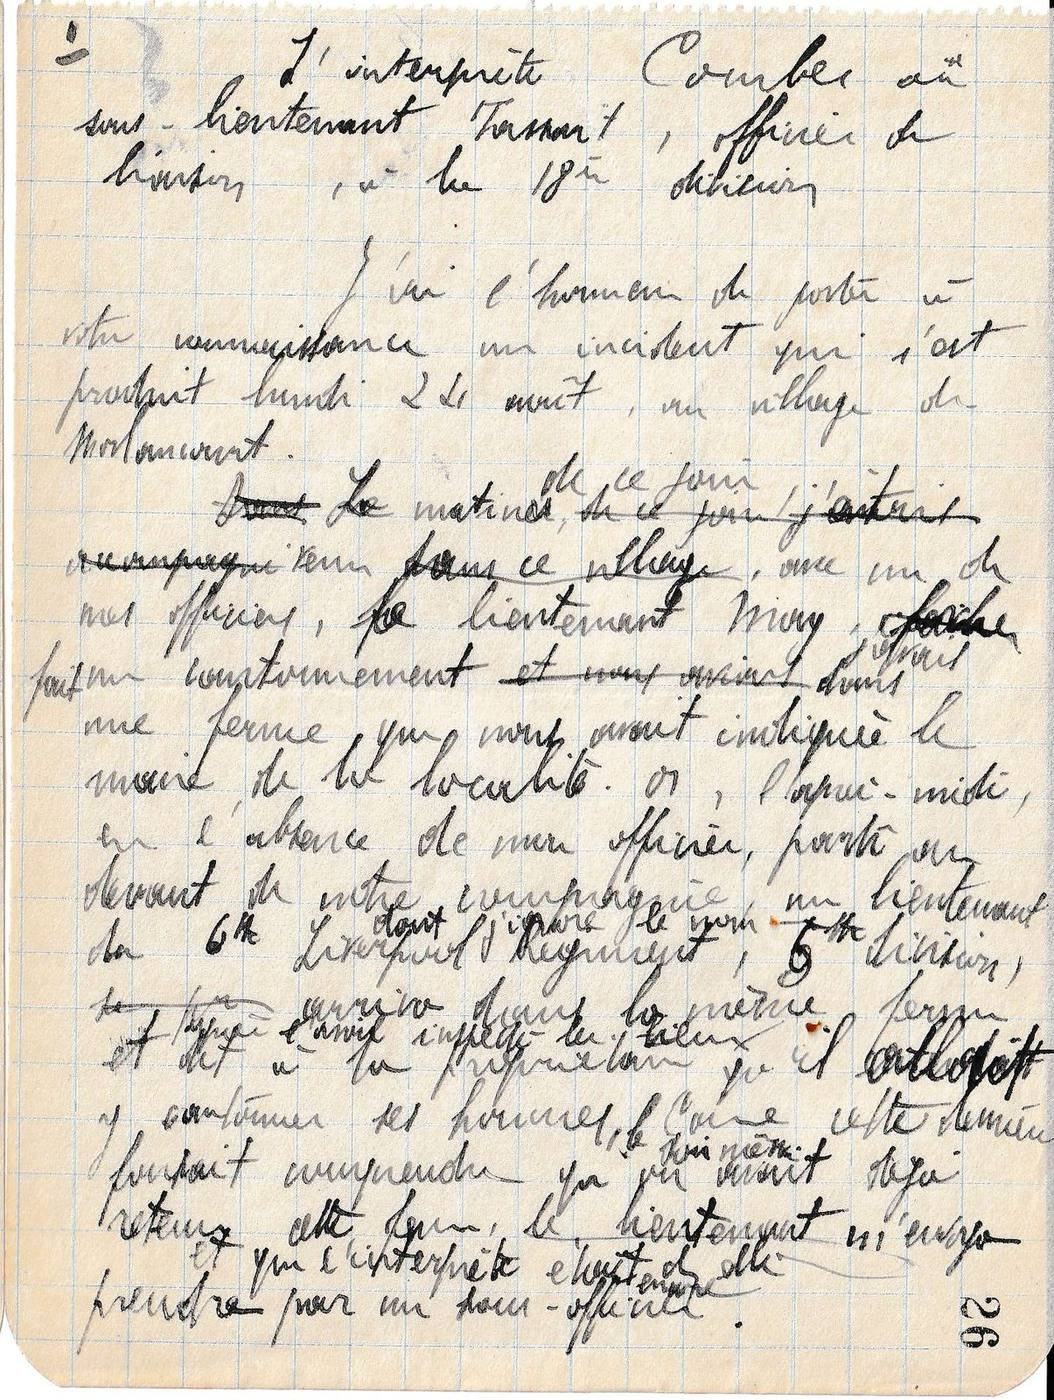
\includegraphics[width=0.78\textwidth,height=0.62\textheight,keepaspectratio]{illustrations/lettres/doc2_incident_p1.jpg}
\caption{Brouillon d'un rapport de l'interprète Hippolyte Combes au sous-lieutenant \LJinc{Tassart}, officier de liaison à la…, première page (archives familiales).}
\end{figure}

Trois feuillets détachés d'un même carnet de poche à papier quadrillé bleu (carreau d'environ 6,3~mm, soit un quart de pouce : carnet vraisemblablement anglais), d'environ 160 × 121~mm, à bord de détachement dentelé et coins arrondis ; ils portent les folios imprimés 26, 27 et 37, mais Combes les a utilisés en travers, si bien que le folio se trouve couché en bas à droite du texte. Il les a numérotés lui-même « 1 », « 2 » et « 3 » dans l'angle supérieur gauche. Le fichier numérique compte deux vues : la première montre les pages 26 et 27, côte à côte (le bord droit de la p.~26 est rogné d'environ 1,5~mm, sans perte de texte) ; la seconde, la page 37. Chaque feuillet n'est écrit que d'un côté, du moins dans ce que montre la numérisation. Les pages 26 et 27 sont le brouillon d'un rapport ; la page 37 est la fin d'une minute de lettre adressée à un « Monsieur le Président ». Le texte, écrit d'un premier jet à l'encre gris-noir pâle, a été repris à l'encre noire, plus dense, qui biffe, surcharge et ajoute dans l'interligne (p.~26, « 6\textsuperscript{th} », « j'avais », « dans », « comptait » ; « fait », en marge, est gris ; p.~27, « de chercher », « cantonnement », « J'élevai » ; p.~37, les longues ratures du milieu de la page). Ratures et surcharges rendent illisibles plusieurs mots du premier jet. Bon état ; quelques petites taches de rouille (p.~26 et 37). Le destinataire du rapport est l'officier français de liaison auprès de la 18\textsuperscript{e} division britannique. Son nom commence par une capitale qui a la forme du T de Combes (haste et barre de tête ondulée, sans barre médiane ni descente sous la ligne, alors que son F en a une) ; viennent ensuite un a, deux hautes boucles (ss), un a ou un o, un n ou un r, puis, détaché, un t barré. On lit donc « Tassart » (ou « Tassant », « Tasson t »), lecture incertaine ; la lecture antérieure, « Ferran », ne rend compte ni de l'initiale ni des deux hautes boucles, et le nom n'a pas été retrouvé dans le \textit{Livre-Journal}. La date est elle aussi incertaine (voir la note) : le 6\textsuperscript{th} Liverpool Regiment appartenait à la 5\textsuperscript{e} division jusqu'en janvier 1916, ce qui plaide pour la fin de l'été 1915, plutôt que pour mars 1916, date avancée par l'édition antérieure. Combes ayant numéroté le feuillet de la p.~37 « 3 », la minute à « Monsieur le Président » faisait sans doute suite aux feuillets 1 et 2, sur une autre page, ou bien ses deux premiers feuillets sont perdus ; le destinataire, qu'on prie d'intervenir « à qui de droit » en faveur de l'indemnité des interprètes, n'est pas identifié (président d'une association professionnelle ou d'une commission parlementaire ?). La signature « H. C. », suivie de la qualité biffée « prof. au coll. » et de « Nogent-le-R. », montre que Combes écrit aussi en tant que professeur du collège de Nogent-le-Rotrou. Les blancs et la disposition du brouillon ne sont pas reproduits ; les ajouts interlinéaires sont placés au point d'insertion le plus probable.

\subsubsection*{1. Rapport sur l'incident de Morlancourt (feuillets 1 et 2, p.~26--27 du carnet)}

\begin{LJlettre}
[p. 1] [\textit{en marge supérieure gauche :}] 1

L'interprète Combes au sous-lieutenant \LJinc{Tassart}\footnote{Lecture incertaine. T de tête, a, deux hautes boucles (ss), a ou o, n ou r, t barré détaché : \textit{Tassart}, \textit{Tassant} ? L'édition antérieure lit « Ferran », que l'initiale (sans barre médiane et sans jambage sous la ligne) et les deux hastes ne permettent pas. Le nom ne figure pas dans le \textit{Livre-Journal}.}, officier de liaison, à la 18\textsuperscript{e} division

J'ai l'honneur de porter à votre connaissance un incident qui s'est produit lundi 2\LJinc{2} \LJinc{aout}\footnote{Après un 2 bouclé, le second chiffre est un 2 (ou un 3) suivi d'un petit trait détaché ; le mois commence par trois jambages et finit par un t barré : « aout » sans accent (comparer « Aout » dans le \textit{Livre-Journal}), plutôt que « mars », qui n'a pas de t, ou « mai ». Le 23 août 1915 est un lundi (le 22 est un dimanche) : à cette date, la 18\textsuperscript{e} division, débarquée en juillet, prenait ses cantonnements dans la vallée de l'Ancre, au contact de la 5\textsuperscript{e} division, dont relevait alors le 1/6th King's (voir la note suivante). Le 2 août 1915 est lui aussi un lundi, si le second signe n'est pas un chiffre. Ni le quantième ni l'année ne sont donc assurés.}, au village de Morlancourt\footnote{Morlancourt (Somme), entre l'Ancre et la Somme, à 6~km au sud d'Albert ; zone de cantonnement des divisions britanniques du secteur de Bray--Fricourt en 1915--1916.}.

\LJdel{\LJinc{Avant}} \LJdel{Le} La matinée, \LJdel{de ce jour} \LJadd{de ce jour} j'\LJdel{\LJinc{étais}} \LJdel{accompagné} venu \LJdel{dans ce village}\footnote{« accompagné » et « étais » sont biffés à l'encre noire ; « dans ce village » est barré par un trait gris ondulé, du premier jet. « venu », non biffé, est maintenu par la correction : le texte corrigé se lit « La matinée de ce jour, venu avec un de mes officiers, le lieutenant May, j'avais fait un cantonnement dans une ferme \ldots ». Le « j' » qui précède « étais » est traversé par le trait gris qui biffe « de ce jour » et devait tomber avec lui.}, avec un de mes officiers, \LJdel{le} le lieutenant May\footnote{Officier de la compagnie d'\textit{Army Service Corps} à laquelle Combes est attaché (152nd Company, train divisionnaire de la 18\textsuperscript{e} division) ; non identifié par ailleurs.}, \LJdel{faire} \LJadd{j'avais} [\textit{en marge gauche :}] \LJadd{fait} un cantonnement \LJdel{et nous avions} \LJadd{dans} une ferme, que nous avait indiquée le maire de la localité. Or, l'après-midi, en l'absence de mon officier, parti au devant de notre compagnie, un lieutenant du 6\textsuperscript{th} Liverpool Regiment\footnote{« 6\textsuperscript{th} » est récrit à l'encre noire. Le 1/6th (Rifles) Battalion du King's (Liverpool Regiment), bataillon de la Territorial Force, fit partie de la 15\textsuperscript{e} brigade de la 5\textsuperscript{e} division de février 1915 à janvier 1916, date de son passage à la 55\textsuperscript{e} division (West Lancashire).}, \LJadd{dont j'ignore le nom} (5\textsuperscript{th}\footnote{Le 5 semble surcharger un 6, à l'encre noire.} division), \LJdel{\LJinc{le fer}} arriva dans la même ferme et \LJadd{\LJinc{après} avoir inspecté les lieux}\footnote{« après », gris, est écrit dans l'interligne et n'est pas biffé ; « avoir », noir, commence par un trait d'attaque qui peut faire lire « l'avoir ».} dit à la propriétaire qu'il \LJdel{\LJill{}} comptait\footnote{« comptait » est écrit à l'encre noire sur un mot du premier jet devenu illisible.} y cantonner ses hommes, \LJadd{\LJinc{le}} Comme cette dernière faisait comprendre \LJadd{\LJinc{lui-même} :} qu'on avait déjà retenu cette ferme \LJadd{et que l'interprète était \LJinc{chez elle}}, le lieutenant m'envoya prendre par un sous-officier.

[p. 2] [\textit{en marge supérieure gauche :}] 2

et \LJdel{me \LJinc{donner}} \LJadd{\LJinc{chez}} \LJdel{\LJinc{l'ordre}} et me donna l'ordre \LJdel{de} \LJdel{\LJinc{fuir}} \LJdel{à la} \LJdel{\LJill{2}} \LJadd{de chercher} \LJdel{\LJinc{que}} un autre cantonnement\footnote{Passage très raturé. Le premier jet, gris, est barré à l'encre noire ; « chez » (?), au-dessus de la ligne, est noir ; « de chercher » et « cantonnement » sont écrits à l'encre noire, en surcharge.}. \LJdel{\LJill{}} J'élevai \LJadd{\LJinc{mais polie}} une protestation ferme. mais respectueuse l'officier \LJinc{s'écria} sur un ton dédaigneux : « this `billet' is all right for me, it shall be mine. --- I don't want to discuss with an interpreter.\footnote{« Ce cantonnement me convient très bien, il sera à moi. Je ne veux pas discuter avec un interprète. » \textit{Billet} : cantonnement chez l'habitant.} » Je n'insistai \LJinc{plus} et m'éloignai aussitôt.

\LJdel{\LJinc{Mais}} deux jours plus tard, mon capitaine a reçu une plainte dans laquelle l'officier \LJadd{\LJinc{sans doute}} en question prétend que j'ai été insolent et que je ne l'ai pas salué. Je proteste contre ces deux allégations avec la plus grande énergie.

[Je ne vous avais pas mis au courant de ces faits, car je ne croyais pas que l'incident auraient de suites]

H. Combes,

A.S.C.\footnote{\textit{Army Service Corps}, le service du train et du ravitaillement de l'armée britannique.} etc
\end{LJlettre}

\subsubsection*{2. Fin d'une minute de lettre à « Monsieur le Président » (feuillet 3, p.~37 du carnet)}

\begin{LJlettre}
[p. 3] [\textit{en marge supérieure gauche :}] 3

\LJdel{Nous sommes très utiles} Les Anglais \LJdel{qui} ne sauraient se passer de nous, car très peu \LJadd{d'entre eux} parlent assez \LJadd{bien} le français pour se faire comprendre. Ils sont les premiers à reconnaître les grands services que nous leur rendons \LJdel{\LJinc{Nous rendons aussi à la cause commune}} \LJdel{et} nous contribu\LJinc{ons} \LJdel{\LJill{}} \LJinc{à la défense nationale} \LJdel{\LJill{}} \LJinc{Ils} \LJdel{\LJill{}} \LJinc{servent extrêmement}\footnote{Deux lignes et demie raturées à l'encre noire, sur un premier jet gris en partie récrit ; ce qui reste lisible est donné sous réserve.}

\LJinc{par la} \LJinc{Aussi}, \LJadd{\LJinc{aussi}} Monsieur \LJadd{donc} le Président, si vous voulez bien vous intéresser à \LJdel{notre} \LJadd{nous} \LJdel{sort} et faire valoir \LJadd{à qui de droit} les considérations qui militent en faveur du maintien de \LJadd{intégral}\footnote{« intégral » est écrit sous la fin de la ligne, à droite ; « faible », sous « indemnité ». La place de ces deux ajouts reste incertaine : « maintien intégral de notre faible indemnité ».} notre \LJadd{faible} indemnité.

Daignez agréer, Monsieur le Président, avec toutes mes excuses pour mon importunité ; l'hommage de mon très profond respect

[\textit{à gauche :}] Interprète H. C

etc.

[\textit{à droite :}] H. C.

\LJdel{prof. au coll.} \LJinc{de}

Nogent-le-R.\footnote{Nogent-le-Rotrou (Eure-et-Loir), où Combes était professeur d'anglais au collège avant la guerre. La formule biffée développe « professeur au collège de ».}
\end{LJlettre}


\subsection{Lettre d'Hippolyte Combes à sa sœur Françoise (destinataire très probable), carmélite à Périgueux, « Au front », vendredi 16 juin 1916}
\phantomsection\label{annexe:doc3}
\begin{figure}[tbp]\centering
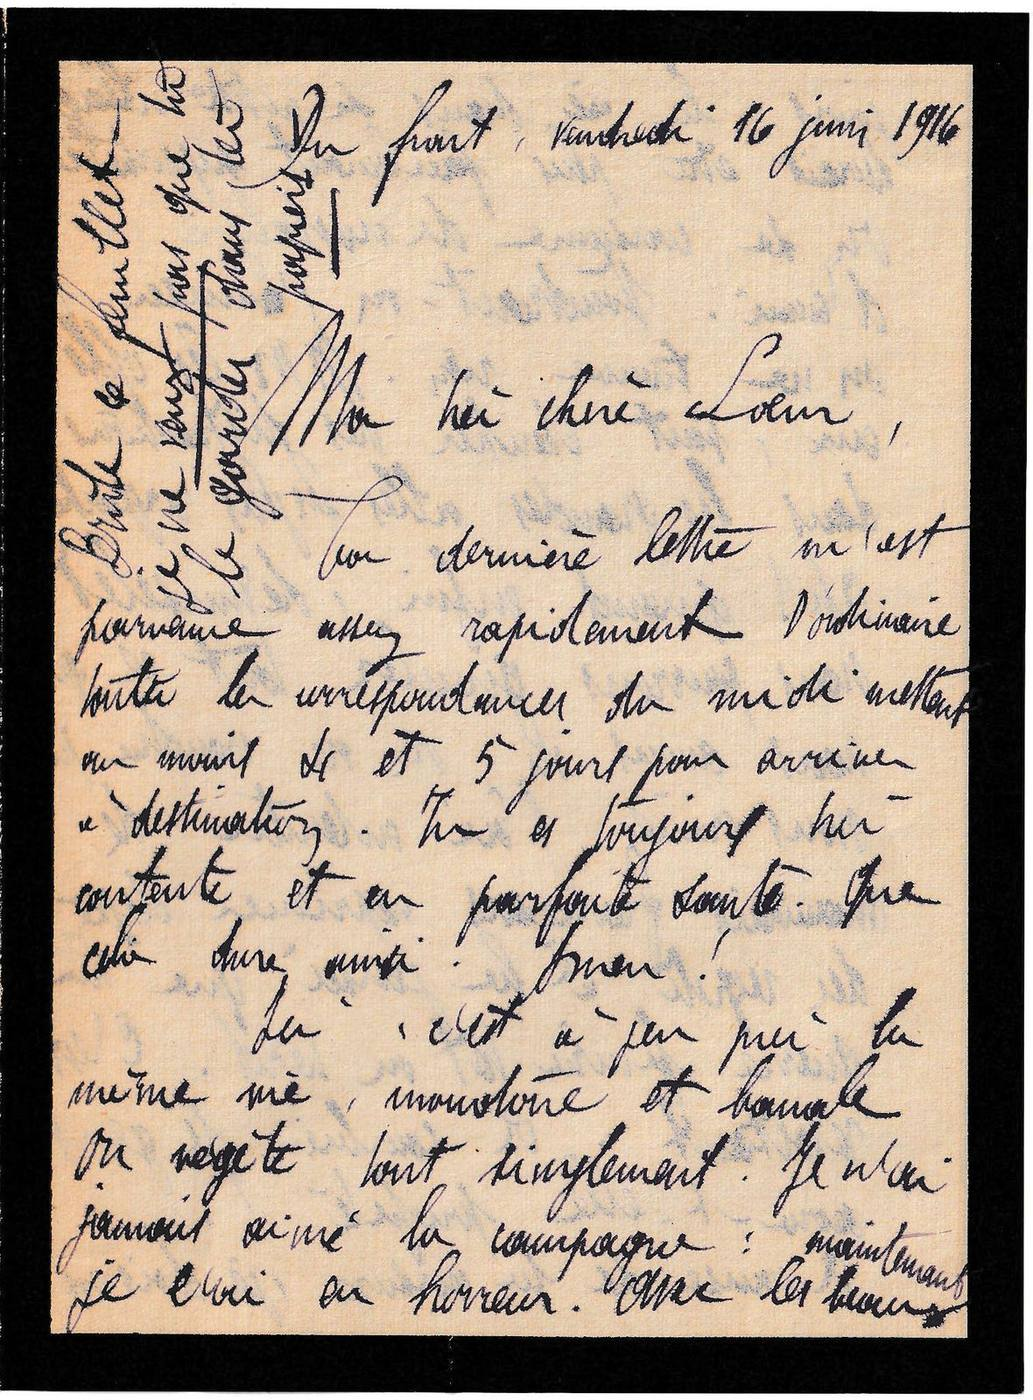
\includegraphics[width=0.78\textwidth,height=0.62\textheight,keepaspectratio]{illustrations/lettres/doc3_juin_1916_p1.jpg}
\caption{Lettre d'Hippolyte Combes à sa sœur Françoise (destinataire très probable), carmélite à Périgueux, « Au front », vendredi 16 juin 1916, première page (archives familiales).}
\end{figure}

Lettre autographe signée « Hippolyte », de quatre pages, sur une feuille double (bifeuillet plié en deux) de papier crème à fin grain toilé ; chaque page mesure environ 12,5 × 16,8~cm (mesure prise sur la numérisation à 300~dpi), et chacune est entourée d'une bordure noire d'environ 7~mm, y compris le long du pli, où le noir est rompu par la cassure du papier : c'est selon toute apparence un papier de deuil, ce qui s'accorderait avec le deuil de Joséphine, sœur de l'auteur (morte en octobre 1914 selon la tradition familiale), sans que rien dans la lettre ne le dise. Le fichier numérique compte deux vues, chacune montrant une face entière du bifeuillet : la vue 2 donne la face extérieure (p.~4 à gauche, p.~1 à droite), la vue 1 la face intérieure (p.~2 et p.~3) ; les fac-similés sont rangés dans l'ordre de lecture. De douze lignes (p.~1, sous la date et l'appel) à dix-neuf lignes par page, d'une cursive rapide et appuyée, sans rature, à l'encre noir-violet (plume à tremper) : là où la plume s'épuise, le trait aminci laisse voir la teinte violette de l'encre (fin de « nostalgie » et « et », p.~2, l.~3 ; « president », p.~4, l.~8), sans changement d'encre, le mot suivant reprenant la teinte foncée. Deux ajouts marginaux, perpendiculaires au texte : à la p.~1, le long du bord gauche, lu de bas en haut, l'ordre de brûler la lettre ; à la p.~4, le long du bord gauche, lu de haut en bas, la formule finale et la signature. Bon état ; transparence du verso, qui laisse voir l'écriture de l'autre face ; une petite tache orangée à la p.~2. La lettre est un original au net, envoyé : sa destinataire l'a gardée malgré la consigne de la p.~1, et elle est revenue ensuite dans les papiers de famille. \textbf{Destinataire.} La lettre s'adresse à « Ma très chère Sœur » et ne la nomme pas. Le titre du fichier (« à sa sœur Joséphine ») est erroné : Joséphine était morte avant le 30 septembre 1916, puisque le \textit{Livre-Journal} l'évoque ce jour-là comme une défunte (« au souvenir de notre gd ami \& de Josephe », cliché 057), et la tradition familiale place sa mort à Nogent-le-Rotrou en octobre 1914. Des sœurs d'Hippolyte, Maria était morte à Carthage en 1903 ; la seule qui vécût encore en 1916 est Françoise (1871--1942), carmélite à Périgueux sous le nom de Sœur Marie de la Croix. Le texte s'accorde avec une religieuse cloîtrée (« Tu es toujours très contente et en parfaite santé. Que cela dure ainsi. Amen ! » ; « Ne m'écris qu'une fois par mois »), sans le prouver : aucun détail ne nomme ni le Carmel ni Périgueux, et l'enveloppe n'est pas conservée. Le destinataire est donc Françoise \textit{par élimination}, sous réserve de l'exactitude de la liste des enfants Combes, établie d'après les papiers de famille et non d'après l'état civil : identification très probable, non certaine ; l'édition antérieure l'affirmait sans réserve. \textbf{Contexte.} En juin 1916, la 18th Division, à laquelle appartient la 152nd Company de l'Army Service Corps, se prépare à l'offensive de la Somme, qui commence le 1\textsuperscript{er} juillet ; Combes vit dans les villages de l'arrière (« la vie dans de petits villages »). La lettre, qui redoute la censure postale et demande d'être détruite, a un ton d'amertume et de révolte que le \textit{Livre-Journal}, commencé quelques semaines plus tard, ne retrouve qu'en passant (« Réflexions amères », 25 août 1916, cliché 028). La transcription respecte l'orthographe, l'accentuation et la ponctuation de l'original : les accents que Combes pose souvent à droite de leur lettre sont rendus quand un trait les porte, et omis quand aucun trait n'est visible (\textit{vegète}, \textit{dejà}, \textit{president}). Les alinéas sont ceux de l'original, marqués par un retrait.

\begin{LJlettre}
[p.~1]

[\textit{en marge gauche, verticalement, de bas en haut, le long de la date et de l'appel :}] Brule\footnote{Sans accent circonflexe : aucun trait au-dessus du u. L'édition antérieure : « Brûle ce feuillet — Je ne veux pas \ldots{} papiers. »} ce feuillet je ne \LJsl{veux pas}\footnote{Un seul trait souligne « veux » et presque tout « pas ».} que tu le gardes dans tes \LJsl{papiers}\footnote{Le trait final de « feuillet » est la barre du t prolongée, non un tiret ; « papiers », sans point, est souligné d'un trait épais séparé. Aucun paraphe ne suit : le trait que l'on a pris pour un paraphe est le A de « Au front ».}

\hfill Au front, vendredi 16 juin 1916

Ma très\footnote{Mot réduit (t, r confondus, s final en trait) mais surmonté de son accent ; l'édition antérieure lit « bien ». Dans « Sœur », la cursive ne permet pas de distinguer la ligature œ de o et e liés.} chère Sœur,

Ta dernière lettre m'est parvenue assez rapidement D'ordinaire toutes les correspondances du midi\footnote{Les lettres venant du Midi de la France. Périgueux, où vivait Françoise, est à plus de 600~km du front de la Somme.} mettent au moins 4 et 5 jours pour arriver à destination. Tu es toujours très contente et en parfaite santé. Que cela dure ainsi. Amen !

Ici, c'est à peu près la même vie, monotone et banale On vegète tout simplement. Je n'ai jamais aimé la campagne : maintenant je l'ai en horreur. Avec les beaux [p.~2] jours, la vie dans de petits villages devrait être plus facilement supportable On se consume de nostalgie et\footnote{La fin de « nostalgie » (\textit{gie}) et « et » sont d'un violet pâle : trait aminci d'une plume presque sèche, non une autre encre ; « d'ennui », après reprise d'encre, est de nouveau foncé. Même effet sur « president » (p.~4).} d'ennui. Voudrait-on s'amuser ? on ne trouve rien. MM\footnote{« Messieurs ». Pas de point abréviatif.} les offs\footnote{« Officiers », abréviation familière du langage des soldats.}, eux, vont chercher des distractions dans les grandes villes les plus rapprochées. Ah ! quand enfin, démuselés, nous pourrons gueuler tout ce que nous avons vu\footnote{Pas de virgule distincte après « vu » : le trait qui descend de l'u se confond avec la boucle du J de « J'ai » (ligne suivante). L'édition antérieure : « vu, on ne voudra pas ».} on ne voudra pas nous croire. J'ai entendu de mauvais Français exprimer dejà du regret à la pensée que la guerre finira tot ou tard. C'est révoltant. A combien de gens aura-t-elle profité ?.. A cause de la censure\footnote{Le contrôle postal militaire, qui lisait et caviardait les lettres envoyées du front. L'injonction marginale de la p.~1 répond à la même crainte.}, je dois me taire.

[p.~3]

A Toulouse\footnote{Combes, qui avait été élevé à Toulouse, y est donc passé récemment, sans doute en permission ; ce séjour n'est pas daté.}, j'ai retrouvé des camarades en permission -- nous avons causé, j'ai constaté avec plaisir qu'ils pensent absolument comme moi. Mon ami, le docteur de \LJinc{L}.\,—\footnote{Initiale calligraphique à boucle haute et boucle basse fermée, de même forme que le L de « Labarthe » dans le \textit{Livre-Journal} (cliché 057) mais aussi que le S de « Si » (p.~4) : L probable, S non exclu ; B (édition antérieure) exclu. On peut penser à Mme de Labarthe, « gde amie affectueuse \& attachée » de Combes à Toulouse (\textit{Livre-Journal}, 29 septembre 1916, cliché 056 ; voir aussi les clichés 057, 060, 135, 137, 138), dont le fils serait ce docteur ; rapprochement hypothétique.}, dont la mère m'est tant\footnote{L'édition antérieure lit « tout ». Le mot a la forme de la fin de « autant » (même page) ; « tout » s'écrit chez Combes avec un o fermé et une longue barre de t.} dévouée, disait : Jamais un officier n'entrera dans mon salon, après la guerre !.. Sa mère et sa jeune femme, après l'avoir ecouté, l'approuvaient tu penses si je faisais chorus\footnote{Aucun signe entre « penses » et « si » : la grande boucle qui s'y trouve est la tête du T de « Tu » (ligne suivante). L'édition antérieure : « l'approuvaient en pensées, et je faisais chorus ».}

Tu sais\footnote{Lecture sûre : T cursif d'un seul trait, puis s, a, i, s. L'édition antérieure : « En tout ».}, nous en avons tous plus qu'assez de cette vie qui se prolonge Pour ma part, j'aimerais autant être sous terre que de rester encore une année en esclavage On est aigri, decouragé, [p.~4] on ne prend \LJinc{goût}\footnote{Un pâté d'encre couvre le t et la place où Combes pose l'accent circonflexe.} à rien. Toutes ces abstractions\footnote{Pas de deux-points : le seul point visible après « abstractions », à hauteur d'œil, est celui du i, déporté vers la droite. L'édition antérieure : « abstractions : gloire, honneur etc. ».} gloire, honneur etc quel tas de blagues ! Vivre avant tout. Dans la mort, il n'y a plus d'alliés ni d'ennemis\ldots\footnote{Trois signes : un point, un tiret court, un point.} Être gouverné par 1 empereur, un roi, ou n'avoir qu'un vulgaire president c'est kif-kif\footnote{« C'est la même chose », de l'arabe \textit{kif} (« comme ») : argot militaire répandu par l'armée d'Afrique. Le long trait qui suit est le délié final du f, non un tiret.} On paie les impost\footnote{Sic, pour « impôts » : i, m, p, o, s long, t barré ; ni s final ni accent.} — et puis qu'on nous f.\footnote{Euphémisme pour « foute » (« qu'on nous fiche la paix »).} la paix, tonnerre de — diable !

Je vais bien. Ne m'écris qu'une fois par mois, c'est plus qu'assez. Si tu savais avec quelle indifférence je parcours tes pages

Je me fous de tout et de tous — Je ne demande que la liberté ou la mort

[\textit{en marge gauche de la p.~4, verticalement, de haut en bas :}] Bien à toi, quand même\footnote{Le trait épais qui prolonge « même » est un délié tiré sans lever la plume, non un tiret ; le trait fin oblique sous « même » est l'attaque du H. L'édition antérieure : « quand même — ».} Hippolyte
\end{LJlettre}


\subsection{Poème anglais signé « Beatrice Chilcott, Wesley Band of Hope », copie de la main d'Hippolyte Combes (attribution probable), sans destinataire, sans lieu ni date}
\phantomsection\label{annexe:doc4}
\begin{figure}[tbp]\centering
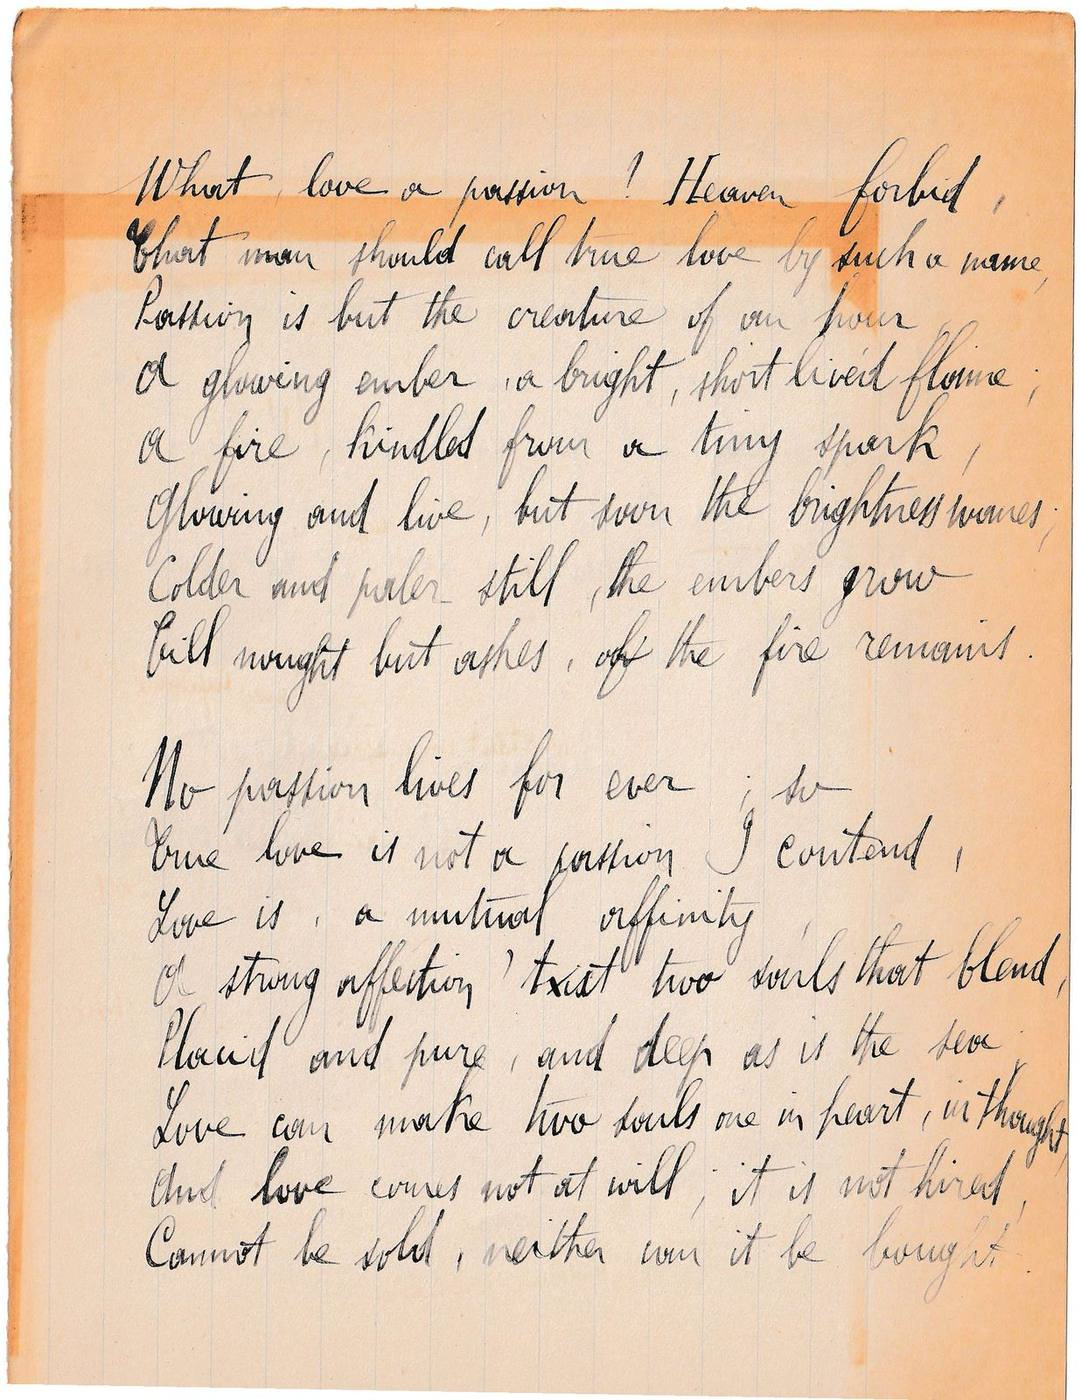
\includegraphics[width=0.78\textwidth,height=0.62\textheight,keepaspectratio]{illustrations/lettres/doc4_poeme_p1.jpg}
\caption{Poème anglais signé « Beatrice Chilcott, Wesley Band of Hope », copie de la main d'Hippolyte Combes (attribution probable), sans…, première page (archives familiales).}
\end{figure}

Copie au net d'un poème anglais sans titre de vingt-quatre vers (trois strophes de huit), suivi de l'attribution « Beatrice Chilcott / Wesley Band of Hope ». Une feuille de papier réglé (lignes fines bleu-gris espacées d'environ 8~mm), large d'environ 155~mm et haute d'au moins 202~mm (le bord inférieur sort du champ de la numérisation), utilisée en travers : les vers coupent la réglure à angle droit. Deux pages écrites, selon toute vraisemblance le recto et le verso (même papier, même réglure, texte continu ; la transparence est trop faible pour le démontrer) : p.~1, strophes 1 et 2 séparées par un blanc ; p.~2, strophe 3 puis, à droite, l'attribution sur deux lignes, le bas de la page restant blanc. Le fichier numérique compte trois vues : la vue 2 reproduit une seconde fois la p.~1 (identique au pixel près), la p.~2 est la vue 3. Encre noire, plume à tremper (traits tour à tour chargés et pâlis : \textit{bought}, \textit{unfathomed}) ; ni rature ni correction. Bon état ; bords brunis ; une bande orangée en équerre (trace d'adhésif ou de contact ?) barre le haut de la p.~1 (v.~1--3) sans gêner la lecture. L'attribution est de la même main et de la même encre que le poème (B de \textit{Beatrice} et de \textit{Beside}, C de \textit{Chilcott} et de \textit{Colder}, W de \textit{Wesley} et de \textit{Which}, H de \textit{Hope} et de \textit{Heav'ns}) : ce n'est pas une signature autographe, mais le nom de l'auteur recopié avec le texte. Le copiste écrit à la française : espace devant « ! » et « ; », ſ long pour le premier s de ss (\textit{passion}, \textit{brightness}, \textit{bitterness}) et à l'initiale (\textit{should}, \textit{sweetens}), T dont la barre se réduit à une boucle (comme dans « Ta », lettre du 16 juin 1916), A en a agrandi, I en forme de J, accent posé à droite de sa lettre (\textit{livéd}) ; s'y ajoutent deux fautes de copie (\textit{'txiat}, \textit{off}). Ce sont les traits de la main d'Hippolyte Combes (voir l'introduction, « L'écriture et la langue du carnet ») : l'attribution est probable, non certaine, faute d'autre texte anglais calligraphié de sa main pour la comparaison. Le poème n'a pas de destinataire. Il est attribué à Beatrice Chilcott, d'une \textit{Band of Hope} rattachée vraisemblablement à une chapelle méthodiste wesleyenne ; elle n'est pas identifiée et le poème n'a pas été retrouvé imprimé (recherche sommaire sur le premier vers). Sans date ni lieu, la feuille est conservée avec les lettres de guerre ; elle a pu être copiée pendant le service de Combes auprès de l'armée britannique, où il assiste par exemple, le 17 septembre 1916 à Raincheval, à un office wesleyen (\textit{Livre-Journal}, cliché 044, l.~17 : « assisté church service (Wesleyans ds petite salle en face eglise village) ») ; ce rapprochement reste une hypothèse. La transcription suit les vers et les strophes ; ſ est rendu par s ; l'espace laissé devant « ! » et « ; » est conservé, les virgules, souvent détachées, sont rattachées au mot qui précède.

\begin{LJlettre}
\noindent What, love a passion ! Heaven forbid,\\
That man should call true love by such a name,\\
Passion is but the creature of an hour\\
A glowing ember, a bright, short livéd\footnote{Un court trait oblique, isolé, surmonte la jonction de e et de d : accent de l'e, posé à droite de sa lettre comme les points et accents de Combes ; il marque la finale prononcée (\textit{liv-ed}), usage de la langue poétique, où l'on attendrait plutôt un accent grave (\textit{livèd}) ; le trait monte vers la droite, comme un aigu. L'édition antérieure l'omet.} flame ;\\
A fire, kindled from a tiny spark,\\
Glowing and live, but soon the brightness wanes ;\\
Colder and paler still, the embers grow\\
Till nought but ashes, \LJinc{off}\footnote{Pour \textit{of}. Le f complet (boucles haute et basse) est suivi d'une haste courte, moitié moins haute qu'un t, terminée en tête par un pâté et traversée par le trait de sortie : second f inachevé, plutôt que t (\textit{oft}), que la hauteur ne soutient pas ; les autres \textit{of} (v.~3, 18 et 21 ; \textit{Band of Hope}) n'en ont pas. L'édition antérieure lit \textit{of}.} the fire remains.

\medskip
\noindent No passion lives for ever ; so\\
True love is not a passion I contend,\\
Love is, a mutual affinity,\\
A strong affection 'txi\LJinc{a}t\footnote{Sic, pour \textit{'twixt} (« entre », forme poétique de \textit{betwixt}). Aucun w : la deuxième lettre est un x croisé, très appuyé ; la quatrième, boucle fermée par un jambage droit appuyé, a la forme du a de \textit{that} (même vers) ; un x cursif, inconnu par ailleurs dans cette main, n'est pas exclu (« 'txixt »). L'édition antérieure normalise en \textit{'twixt}.} two souls that blend,\\
Placid and pure, and deep as is the sea.\\
Love can make two souls one in heart, in thought,\\
And love comes not at will ; it is not hired,\\
Cannot be sold, neither can it be bought.

\medskip
\noindent [p.~2]

\noindent A mystic power, unfathomed still,\\
Which baffles all the probing powers of man\\
Potent, enthralling, it shapes men's destinies,\\
And silent ruled since first the world began ;\\
Heav'ns\footnote{Pour \textit{Heaven's} (« du Ciel ») : une seule apostrophe, entre v et n.} greatest gift, love is the source of life\\
Which sweetens all the bitterness and pain ;\\
And ever points toward the divine love\\
Beside which, human love is poor and vain.

\begin{flushright}
-- Beatrice Chilcott\footnote{La barre des deux t se prolonge en un long délié descendant, continu jusqu'au pâté qui le termine : il n'y a pas de point séparé. L'édition antérieure ponctue « Chilcott, ».}\\
Wesley Band of Hope --\footnote{Les \textit{Bands of Hope}, sociétés de tempérance pour enfants et adolescents nées à Leeds en 1847, étaient le plus souvent rattachées à une église ou à une chapelle ; « Wesley » désigne vraisemblablement une chapelle méthodiste wesleyenne. Voir L.~L.~Shiman, « The Band of Hope Movement: Respectable Recreation for Working-Class Children », \textit{Victorian Studies}, 17/1, 1973, p.~49--74. Beatrice Chilcott n'est pas identifiée.}
\end{flushright}
\end{LJlettre}


\subsection{Correspondance d'Hippolyte Combes à sa femme Marguerite Combes, née Calmels : six pièces (cartes postales), Saint-Pol-sur-Ternoise, Paris et Les Andelys, 12 novembre -- 2 décembre 1918}
\phantomsection\label{annexe:doc5}
\begin{figure}[tbp]\centering
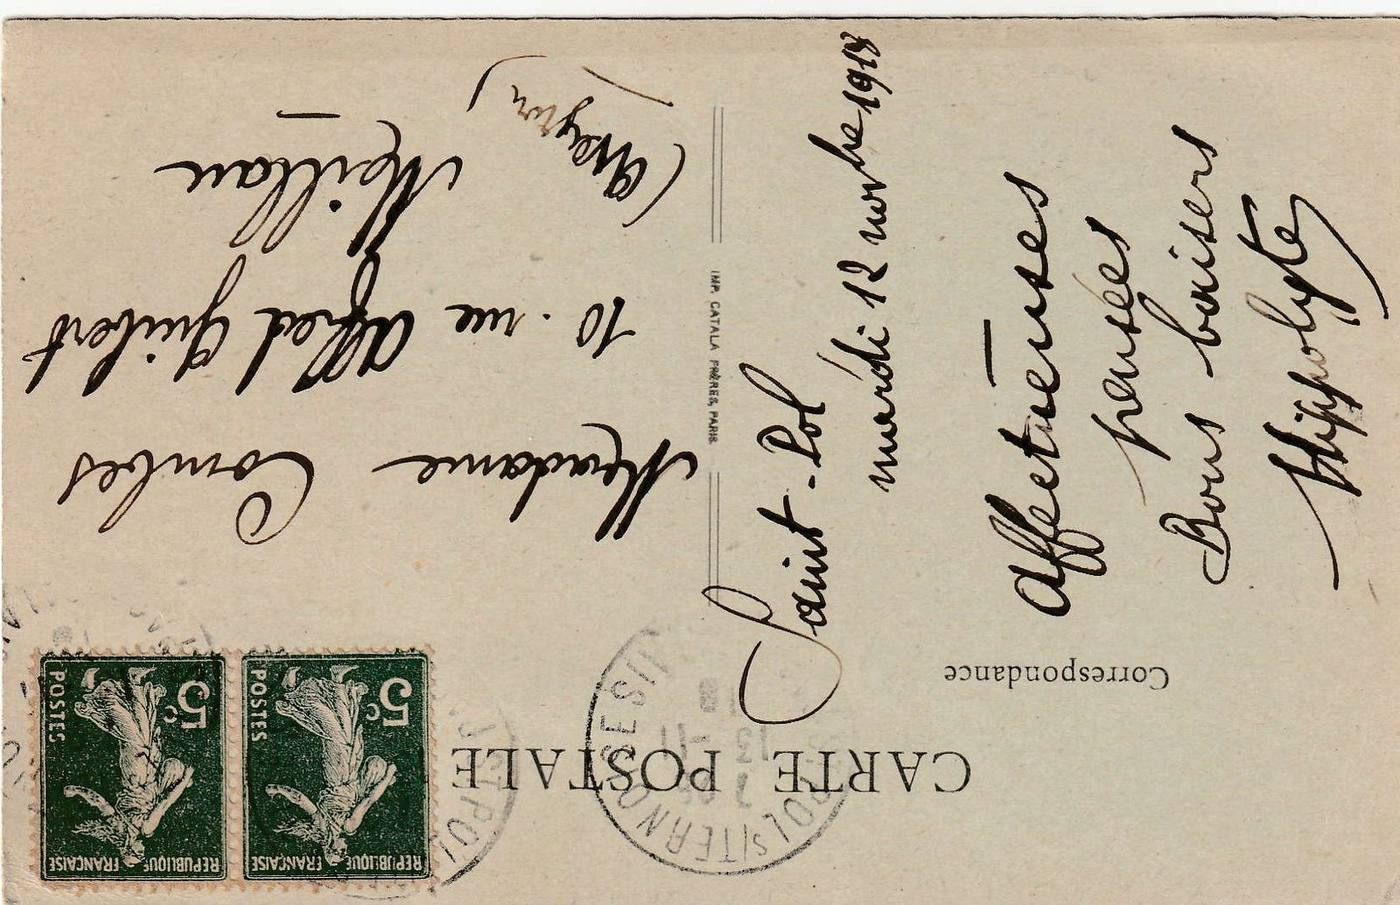
\includegraphics[width=0.78\textwidth,height=0.62\textheight,keepaspectratio]{illustrations/lettres/doc5_novembre_1918_p1.jpg}
\caption{Correspondance d'Hippolyte Combes à sa femme Marguerite Combes, née Calmels : six pièces (cartes postales), Saint-Pol-sur-Ternoise,…, première page (archives familiales).}
\end{figure}

Six pièces autographes d'Hippolyte Combes, toutes écrites sur des cartes postales d'environ 140 $\times$ 89~mm (mesure prise sur les numérisations à 300~dpi, page A4), réparties dans quatre fichiers : une carte isolée de Saint-Pol-sur-Ternoise (12 novembre, au bas de la page du fichier « carte 2 decembre 1918 ») ; deux lettres écrites chacune sur deux cartes numérotées « 1/ » et « 2/ », depuis la Bibliothèque Sainte-Geneviève à Paris (25 et 26 novembre) ; une lettre des Andelys sur deux cartes numérotées « 1 » et « 2 » (28 novembre) ; une carte des Andelys sans date ni signature, décrivant l'église Notre-Dame (fin novembre ou début décembre), numérisée avec la précédente ; une carte des Andelys du 2 décembre. Hormis la carte de Saint-Pol, envoyée à découvert, aucune ne porte d'adresse ni de timbre : elles sont parties sous enveloppe. Combes écrit sur la face de correspondance, en travers (carte tenue en hauteur), sans tenir compte du filet vertical imprimé ; le filet double horizontal imprimé de la carte, qui traverse le texte, n'est pas une rature. Il emploie aussi les marges, où il écrit verticalement (souscriptions, post-scriptum). Les cartes du 25 novembre, de papier chamois (mention multilingue « Carte postale » de l'Union postale universelle, en partie en caractères cyrilliques), sont écrites à l'encre noire virée au brun ; celles du 26, sur cartes illustrées de l'Opéra de Paris (« Le Grand Escalier », éd. E.L.D., n\textsuperscript{os} 4304 et 4306, faces reproduites en p6--p7), à l'encre noire ; celles des Andelys du 28 novembre et la carte non datée, sur cartes illustrées du Grand-Andely (vue générale, portail et flanc gothique de Notre-Dame, la dernière imprimée par A. Lavergne, à Vernon ; faces reproduites en p11--p13), à l'encre très foncée, nettement violette dans les traits fins (« Amen ! ») : c'est l'encre violette de la « chambre civile », que la carte du 2 décembre, tracée, dit-elle, « à l'encre noire » dans la « chambre militaire », oppose à l'autre. La face illustrée de la première carte du 28 novembre porte un cachet à date « LES ANDELYS [EURE] 29-11 18 » sans timbre. Bon état ; bords légèrement rognés par la numérisation, qui ampute la ligne extrême de la marge droite de la carte 1 du 28 novembre. Le fichier du 25 novembre (« lettre à bonne maman ») est une photographie des deux cartes superposées ; l'intitulé du fichier vient de la famille. Le destinataire n'est jamais nommé en suscription, sauf sur la carte de Saint-Pol (« Madame Combes », à Millau, chez les Calmels) ; il est certain : Combes s'adresse à sa femme (« Ma Margueritou tant aimee », « Ton mari qui t'adore », « notre fillette », Valentine, née le 17 septembre 1918, « ton excellente mère »). Le contexte est celui du dernier poste de Combes : relevé de la Mission militaire française près l'armée britannique au lendemain de l'armistice, il est « dirigé le 24 novembre 1918 sur l'École préparatoire des Andelys comme professeur de langue anglaise » (état signalétique et des services), où il est nommé caporal le 4 décembre ; il sera envoyé en congé illimité le 7 février 1919. Il passe par Paris les 25 et 26 novembre et rejoint Les Andelys dans la nuit du 26 au 27.

\subsubsection*{1. Carte postale, Saint-Pol-sur-Ternoise, mardi 12 novembre 1918}

Carte postale (imprimeur : « Imp. Catala frères, Paris »), face d'adresse ; deux timbres Semeuse à 5~c verts ; cachet à date « ST-POL S/TERNOISE / [PAS-DE-CALAIS] » du 13 novembre 1918. Le texte occupe, verticalement, la moitié gauche ; l'adresse, la moitié droite.

\begin{LJlettre}
[\textit{moitié gauche, verticalement :}] Saint-Pol\footnote{Saint-Pol-sur-Ternoise (Pas-de-Calais). Le lendemain de l'armistice.}

mardi 12 nov\LJsup{bre} 1918

Affectueuses

pensées

Bons baisers

Hippolyte

[\textit{moitié droite, adresse :}] Madame Combes

10 . rue Alfred Guibert

(Aveyron) Millau\footnote{Domicile de la famille Calmels, à Millau, où Marguerite Combes a mis au monde Valentine le 17 septembre 1918.}
\end{LJlettre}

\subsubsection*{2. Lettre en deux cartes postales, Paris, lundi 25 novembre 1918}

\begin{LJlettre}
[p. 1] [\textit{en haut, à gauche :}] 1/

Paris, lundi 25 novembre 1918

11 h. matin

Ma Chérie ce matin à 6 h. enfin, je me suis retrouvé dans cette ville que je préfère à toutes les autres capitales du monde. Je ne repartirai que demain, Je n'ai pas voulu descendre chez tes cousines, à Neuilly\footnote{Les Faure : Mme Camille Faure, née Marguerite Barnerot (1874--1954), cousine de Marguerite Combes, veuve, et ses enfants ; ils habitent Neuilly-sur-Seine, rue d'Armenonville (\textit{Livre-Journal}, cl.~130). Voir la lettre du lendemain.}, afin de ne point les déranger et aussi pour me sentir plus libre. Cet après-midi j'irai les voir. Volontiers, si l'on me prie, j'accepterai à déjeuner demain seulement.

Avec plaisir je suis venu au Quartier Latin ; Chargé de souvenirs, il y \LJill{}\footnote{Un mot d'environ huit lettres, repassé à l'encre plus noire et chargée, comme plusieurs mots du bord gauche de cette carte, et brouillé par la mention imprimée « Carte postale » : ductus approximatif « \textit{?eguilbat} » (attaque bouclée, g ou q, u, i, l bouclé, b ou l, a, t). Aucune lecture satisfaisante ; le verbe attendu (« il y [a]… ») ne se laisse pas reconnaître.} pour moi ! Je n'ai pu me loger, faute de place, dans mon hôtel de prédilection, (University Hotel, 160. rue St-Jacques, \LJinc{en} face de l'École de Droit)\footnote{Le premier mot, repassé, peut aussi se lire « Eu » ; la parenthèse fermante est nette, l'ouvrante, devant \textit{University}, fine. Le 160, rue Saint-Jacques est à quelques pas de la place du Panthéon, où se trouvent la Faculté de droit, la Bibliothèque Sainte-Geneviève et l'Hôtel du Panthéon.}. J'ai pris une jolie chambre à l'Hôtel du Panthéon, au 2\LJsup{ème} sur le devant. Tout à l'heure, je me suis débarbouillé et bien reposé. Je t'écris dans la grande salle de la Bibliothèque Geneviève\footnote{Sic, pour Bibliothèque Sainte-Geneviève (place du Panthéon), que Combes fréquentait étudiant (« Tant de souvenirs », lettre du 26) ; la lettre du lendemain donne le nom complet.}. Que de fois Joséphine\footnote{Joséphine Combes (1873--1914), sœur d'Hippolyte, morte à Nogent-le-Rotrou en octobre 1914. L'accent du é est caché par la signature écrite en marge.} m'y a-t-elle accompagné ! Elle lisait à côté de moi. Comme je serais heureux de te posséder, de te sentir

[\textit{dans la marge gauche, verticalement, en colonne :}] Mes plus doux baisers [\textit{puis :}] Ton Petitou\footnote{Hypocoristique (« petit »), comme \textit{Margueritou}, \textit{Perlounette} et \textit{poutous} (« baisers », languedocien \textit{potons}) des lettres suivantes.} qui t'aime \LJinc{si} tendrement Hippolyte

[p. 2] [\textit{en haut, à gauche :}] 2/

tout près de moi ! Courage et confiance, notre séparation finira bientôt.

Ma nouvelle affectation, à défaut d'avantages plus appréciables, aura du moins celui de m'avoir bien rapproché de Paris 102 kilomètres environ)\footnote{Sic : aucune parenthèse ouvrante. Les Andelys (Eure), sur la Seine, sont à une centaine de kilomètres de Paris et à une quarantaine de Rouen.}. Le jeudi ou le dimanche, sans doute, j'obtiendrai facilement des permissions de 24 heures. Ainsi je pourrai me rendre soit à Rouen, soit dans la capitale et aussi --- et surtout, à Nogent-le-Rotrou\footnote{Nogent-le-Rotrou (Eure-et-Loir), dans le Perche, où Combes enseignait avant la guerre.}. J'éprouverai une satisfaction profonde quand je reverrai mon chez moi du Perche quitté depuis près de 4 ans. La maison que j'habite à Nogent (17. rue Saint-Hilaire\footnote{Pas de parenthèse fermante visible : « Saint-Hilaire » touche le bord droit de la carte.} est autrement jolie et pittoresque que celle de Toulouse, rue de Languedoc, 24. Elle a un petit air flamand qui lui donne une certaine originalité.

Santé toujours parfaite. Je ne me suis jamais mieux porté, me semble-t-il. Afin de me \LJinc{ressembler}\footnote{Graphie « re\textit{ſſ}e\ldots{}ler » : r, e, double s long, puis quatre ou cinq jambages et une haste ; « ressembler » donne le seul sens satisfaisant (« pour être, comme moi, en parfaite santé »). L'état antérieur, « Enfin je me ressemble tout à fait, malgré les [illis.] », est une reconstruction.} tout à fait, ménage-toi, sois philosophe et attends sans fièvre les événements. Je ne tarderai plus à recouvrer la liberté entière et définitive. Ne t'alarme point au sujet de notre fillette\footnote{Valentine Combes, née le 17 septembre 1918.}. Elle prendra le dessus et grossira en \LJinc{vitesse}\footnote{Mot empâté : haste initiale (v ou b), i, t, puis s long et e. L'état antérieur lit « à l'aise ».} à partir du 3\LJsup{ème} mois.

[\textit{dans la marge gauche, verticalement :}] Tu peux m'écrire à l'adresse que je t'ai indiquée dimanche.
\end{LJlettre}

\subsubsection*{3. Lettre en deux cartes postales, Paris, mardi 26 novembre 1918}

\begin{LJlettre}
[p. 1] [\textit{en haut, à gauche :}] 1/

Paris, mardi 26 novembre 1918

11 h. matin

Ma Margueritou tant aimee

Me voici de nouveau installé dans la grande salle de la Bibliothèque Sainte-Geneviève. Comme je m'y plais ! Tant de souvenirs me la rendent chère ! Devant moi, sur la table, j'ai des revues françaises et un volume de Maeterlinck. Mais, au lieu de lire, je fais ma petite correspondance J'ai passé une excellente nuit. Je me sens bien reposé. Ce soir, je continuerai et terminerai mon voyage. Je prendrai l'express du Havre\footnote{Ligne Paris--Rouen--Le Havre ; Combes descend vraisemblablement à Gaillon ou à Saint-Pierre-du-Vauvray, gares les plus proches des Andelys.}, à 10\LJsup{H} 15, gare St-Lazare, j'arriverai à destination après minuit. Peu m'importera ! Partant par le dernier train, j'aurai pu rester qq heures de plus dans la capitale\quad Hier, j'ai fait une très longue visite aux Cousines Faure. Marguerite\footnote{Mme Camille Faure, née Marguerite Barnerot (1874--1954), cousine de la destinataire, veuve d'un ingénieur des Ponts et Chaussées ; ses enfants : Henri (1895--1918), André, Germaine (1901--1944) et Marcel (1906--1999).} descendait l'escalier, comme j'arrivais au 2\LJsup{ème} étage. Elle sortait avec ses parentes, les dames Taillandier\footnote{Lecture assez sûre (T-a-i-l-l-a-n-d-i-e-r) ; non identifiées. L'état antérieur : « ses [voisines ?], les dames [illis.] ».}, auxquelles elle m'a présenté. Elle a renoncé à

[\textit{dans la marge gauche, verticalement :}] Mes plus tendres baisers pour toutes deux [\textit{au bas de la marge :}] Ton mari qui t'adore Hippolyte

[p. 2] [\textit{en haut, à gauche :}] 2

la promenade, pour me recevoir. Je l'avais priée de n'en rien faire. Germaine était aussi là, elle préparait ses devoirs.

J'ai pu causer durant plusieurs heures avec Marguerite. Elle m'a raconté son pèlerinage bien triste à Moyenneville\footnote{Moyenneville (Oise), dans le secteur de la bataille du Matz (9--12 juin 1918) : vraisemblablement le lieu de la mort ou de la sépulture d'Henri Faure, tué le 11 juin 1918, le « pauvre défunt » de la phrase suivante.}. Nous avons longuement parlé du pauvre défunt. Toi et notre fillette, naturellement, avez été l'intéressant sujet de nos conversations. Ta Cousine veut t'écrire elle-même ce qu'elle pense et qu'elle te conseillerait. Je suis entièrement de son avis. Je te résumerai en qq mots ce qu'elle m'a dit à propos de notre mignonne Valentine. Tu ne dois point t'inquiéter, ni t'énerver ; avec le temps, l'enfant prendra le dessus et deviendra magnifique, comme le petit Bonhomme, que tu as vu, paraît-il à Paris, chez les locataires du rez de-chaussée 26, rue d'Armenonville\footnote{Lecture nette, appuyée par le \textit{Livre-Journal} (cl.~130 : Neuilly, « rue d'Armenonville », domicile de Mme Faure) ; la rue est à Neuilly, non à Paris intra-muros. La haste qui descend sous « Ar- » appartient au b de « bien » (ligne suivante). L'état antérieur lit « rue d'[Angoulême ?] ».} : il était alors bien chétif, bien menu. Sois calme, patiente et surtout écoute ton excellente mère : apprends à dormir. Le sommeil t'est aussi nécessaire que le lait à la fillette
\end{LJlettre}

\subsubsection*{4. Lettre en deux cartes postales, Les Andelys, jeudi 28 novembre 1918}

\begin{LJlettre}
[p. 1] [\textit{dans l'angle supérieur gauche :}] 1

Les Andelys, jeudi soir 28 Nov\LJsup{bre}\footnote{Le millésime manque ; la fin de la date est en partie couverte par le post-scriptum marginal.}

Ecole \LJsl{Militaire}\footnote{L'École militaire préparatoire des Andelys, école d'enfants de troupe, où Combes vient d'être affecté comme professeur d'anglais.}

Ma jolie Perlounette

Aujourd'hui encore, liberté entière. Je suis allé ce matin à l'École L'emploi du temps, pour l'anglais n'\LJinc{est}\footnote{Fin de ligne couverte par le post-scriptum marginal : n', puis a ou e et un t barré.} pas encore fixé. Jusqu'à présent, on n'enseignait pas cette langue. Quand mon horaire aura été établi, samedi ou lundi, je commencerai mon nouveau service. À ma honte, je l'avouerai le plus tard sera le mieux, je suis nullement pressé. Pour le moment, je jouis en paix d'un repos complet ! Oh ! le paresseux !

Tu sais, il fait délicieux dans ma grande chambre, rue de la sous-préfecture\footnote{Les Andelys sont alors sous-préfecture de l'Eure. Combes loge en ville (« chambre civile ») et dispose aussi d'une « chambre militaire » à l'École (carte du 2 décembre).}. Affalé sur mon fauteuil --- un vieux pouf, --- les jambes sur une chaise, je rumine, je lis et . -- je fume. Horreur, t'écrieras-tu ! Oui, voilà ce que cause le désoeuvrement.

[\textit{dans la marge gauche, verticalement, de bas en haut, en quatre lignes :}] \LJinc{A demain}, Chérie [\textit{puis :}] Reçois mes plus tendres baisers et embrasse bien fort pour moi notre mignonne fillette [\textit{au bas de la marge :}] Ton mari qui t'aime Hippolyte.

[\textit{dans la marge droite, verticalement, de bas en haut ; en haut, à droite de la date :}] Je lis et relis avec une attention \LJinc{heureuse} les articles de journaux relatant [\textit{en bas de la même marge :}] tu dois lire avec passion les récits des marches \LJinc{triomphales de nos troupes} \LJlac{} les fêtes d'Alsace Lorraine, ces chères \LJlac{}\footnote{Post-scriptum en deux blocs. Le premier, serré dans l'angle supérieur droit, s'interrompt sur « relatant » ; le second commence dans l'angle inférieur droit (« Tu dois / lire ») et se poursuit sur la ligne extrême, le long du bord, que la numérisation ampute : « triomphales de nos troupes » est écrit sous « des marches », à demi coupé ; « les fêtes d'Alsace Lorraine, ces chères » est sur la même ligne que « avec passion… marches » et pourrait aussi continuer « relatant » ; la fin (« ces chères [provinces] » ?) est perdue. « heureuse » : h, e, u, puis r et euse comprimés ; on a aussi pensé à « haineuse », peu compatible avec le sujet. Entrées des troupes françaises à Metz (19 novembre) et à Strasbourg (22 novembre 1918).}

[p. 2] [\textit{dans l'angle supérieur gauche :}] 2

Bientôt je te décrirai longuement et la ville et la région. Non loin de ma rue, se trouve l'église\footnote{Notre-Dame du Grand-Andely (\textsc{xiii}\textsuperscript{e}--\textsc{xvi}\textsuperscript{e} siècle), dont la tradition attribue la fondation à un monastère créé par sainte Clotilde.}, admirable ! J'y suis entré déjà plusieurs fois et me suis arrêté sur les trottoirs, (d'en face inlassablement Il y a des vitraux merveilleux, des sculptures ogivales magnifiques. Tout de suite, cette église et\footnote{Sic, pour \textit{est} ; de même plus bas (« et naturellement ») : un s bouclé, comme dans les autres \textit{est} de ces cartes, n'y est pas.} devenue ma passion. Je n'en aurai point d'autre, ici.

A l'École, on reçoit La Revue Revue de Paris\footnote{Sic, sans ponctuation, « Revue » répété en début de ligne. \textit{La Revue} (ancienne \textit{Revue des revues}) et \textit{La Revue de Paris} sont deux périodiques ; une répétition fautive est également possible.} et d'autres revues non moins intéressantes. La bibliothèque assez riche, et naturellement à la disposition des professeurs. J'ai des collègues fort sympathiques. Ce sont tous des universitaires, mobilisés eux aussi. Ils\footnote{« Ils » repassé, peut-être sur un premier « et » ; la suite (« ne désirant ») est restée au participe.} ne désirant qu'une chose : être libérés. Ils appartiennent un peu à toutes les classes. En majorité nous sommes des territoriaux ou de la R.A.T.\footnote{Réserve de l'armée territoriale, qui groupe les classes les plus anciennes. Combes, né en 1876, est de la classe 1896.} Tous nous comptons les jours qui nous séparent de la démobilisation. En ce qui me concerne, ce sera sûrement en janvier au plus tard. Amen !

[\textit{dans la marge gauche, verticalement :}] Il me tarde beaucoup d'avoir de \LJinc{nouveau}\footnote{Mot de six ou sept lettres, à jambages indistincts, suivi d'un long trait : la forme convient à « nouveau » ; le sens (« d'avoir de [X] --- et aussi --- de tes nouvelles ») attendrait un nom de personne, peut-être un surnom de l'enfant (« Nounou » ?).} --. et aussi . de tes nouvelles

[\textit{dans la marge droite, verticalement :}] mille \LJinc{gros} poutous : \LJill{2} \LJinc{Kouine}. bien , bijou.\footnote{Ligne de bord, très empâtée et croisée par les fins de lignes du texte ; après les deux points, deux mots illisibles (un J ou un à, un mot court), puis un mot lu « Kouine » (surnom ?).}
\end{LJlettre}

\subsubsection*{5. Carte postale, Les Andelys, lundi 2 décembre 1918}

\begin{LJlettre}
Ecole Militaire des Andelys,

lundi 2 décembre 1918

Chérie, cette carte, écrite à l'encre \LJsl{noire}, vient directement de ma chambre militaire. Tu le sais, je ne me sers que d'encre violette, dans ma chambre civile. Je ne commencerai pas les cours d'anglais avant demain mardi. Samedi 21\footnote{Samedi 21 décembre 1918, veille des vacances de Noël.} sera le dernier jour de classe de l'année. A mon retour de permission, en janvier, je serai presque à la veille du plus beau, du plus heureux jour de ma vie, celui où je serai enfin démobilisé. Je n'ai jamais autant désiré une chose, depuis que j'existe.\quad Ma santé se maintient inaltérable est-il besoin de le répéter ? Toi aussi, je t'en prie, reste calme, attends sans fièvre les événements que nous réserve demain. Notre séparation n'est plus qu'une question de semaines. Oh ! Dieu, la liberté, je vais donc la recouvrer ! Cette certitude me transporte d'allégresse

Mes plus doux baisers pour Toi et pour la fillette. Ton mari qui t'aime tant Hippolyte
\end{LJlettre}

\subsubsection*{6. Carte postale sans date ni signature, Les Andelys, fin novembre ou début décembre 1918}

Carte numérisée avec la lettre du 28 novembre, sans numéro, sans date, sans formule d'appel ni signature : c'est la suite d'une lettre dont le début et la fin manquent, ou un feuillet isolé d'une autre lettre. Elle développe la description de Notre-Dame annoncée le 28 novembre (« Bientôt je te décrirai longuement… ») et suppose plusieurs visites (« Je commence à connaître cette église dans les moindres détails ») : elle est postérieure au 28 novembre, sans qu'on puisse la placer avant ou après la carte du 2 décembre. Sa face illustrée représente le portail de Notre-Dame.

\begin{LJlettre}
Cette église fait mon admiration. Je suis obligé de m'arrêter toutes les fois que je passe sur la Place Notre-Dame et, après avoir contemplé l'extérieur, je pénètre dans la nef, fais le tour des bas coté, du choeur, sans jamais me lasser. Il y a de merveilleux vitraux, (XIIIe et XIV\LJsup{o}) qui reproduisent les principaux faits de l'existence de S\LJsup{te} Clotilde\footnote{Sainte Clotilde (\textit{c.} 475--545), reine des Francs, femme de Clovis ; la tradition lui attribue la fondation d'un monastère aux Andelys.}. Il y a fresques\footnote{Sic, sans article.}, assez bien conservées. Il y a aussi des sculptures superbes. L'architecture, l'ensemble même de l'édifice retiennent mon attention. Je commence à connaître cette église dans les moindres détails. Plus je la revois, plus je l'aime Je m'y plais autant que dans les plus belles cathédrales de France et d'Angleterre. J'ai acheté toutes les vues qui la représentent, collection de 30 cartes postales ---
\end{LJlettre}
